\documentclass[preprint,12pt]{elsarticle}

\usepackage{amsmath,amssymb,amsthm}
\usepackage{booktabs}
\usepackage{tabularx}
\usepackage{array}
\usepackage{graphicx}
\usepackage{xcolor}
\usepackage{hyperref}

\definecolor{primary}{RGB}{20,75,130}
\hypersetup{
  colorlinks=true,
  linkcolor=primary,
  citecolor=primary,
  urlcolor=primary
}

\newtheorem{theorem}{Theorem}
\newtheorem{proposition}{Proposition}
\journal{SoftwareX}

\sloppy
\begin{document}

\begin{frontmatter}

\title{GeoSolver 2D: An Exact-Aware, Permutation-Invariant Triangle Classification Kernel for Interactive Geometry Software}

\author[1]{Bao-Trung Nguyen\corref{cor1}}
\ead{trungyds16@gmail.com}
\cortext[cor1]{Corresponding author. ORCID: \href{https://orcid.org/0009-0009-5780-3385}{0009-0009-5780-3385}}
\address[1]{Independent Researcher, Ho Chi Minh City, Vietnam}

\begin{abstract}
Interactive geometry software often decides whether a drawn triangle is equilateral, isosceles, or right by comparing floating-point quantities against numerical tolerances. Implemented as an ordered conditional chain, this approach can (i) return conflicting classifications when the same triangle is entered with vertices in a different permutation order, and (ii) label a lattice triangle as equilateral although none exists on $\mathbb{Z}^2$. Neither observation is new mathematics: the second is a textbook consequence of the Gauss--Shoelace formula. We address the software engineering question that follows: how to build an embeddable, dependency-free micro-kernel that is exact whenever its inputs are representable as decimals with at most four fractional digits ($k \le 4$), explicit about when they are not, and invariant under vertex relabelling. GeoSolver 2D returns a geometric type label, an apex, and an epistemic flag stating whether the verdict was obtained by exact integer arithmetic or by tolerance. The continuous tolerance regime provides determinism under relabelling, not higher accuracy than existing heuristics. The implementation is verified across 62 tests (achieving 92\% statement coverage on the headless core suite), an exhaustive $10 \times 10$ integer grid sweep ($943{,}512$ evaluations), a $20 \times 20$ grid comparison against SymPy 1.14, and realistic execution baselines. GeoSolver 2D is released as open-source software under the GNU General Public License v3 (GPLv3).
\end{abstract}

\begin{keyword}
Dynamic Geometry System \sep Triangle Classification \sep Permutation Invariance \sep Integer Lattice \sep Provenance Tracking \sep Software Verification
\end{keyword}

\end{frontmatter}

\begin{table}[!htbp]
\centering
\caption{Code metadata (mandatory).}
\label{tab:metadata}
\small
\begin{tabularx}{\linewidth}{@{}l>{\raggedright\arraybackslash}p{0.33\linewidth}>{\raggedright\arraybackslash}X@{}}
\toprule
\textbf{Nr.} & \textbf{Code metadata description} & \textbf{Metadata} \\
\midrule
C1 & Current code version & v3.2.1 \\
C2 & Permanent link to code/repository used for this code version & \url{https://github.com/trungyds16-coder/geosolver-core} (release tag v3.2.1); archived at \href{https://doi.org/10.5281/zenodo.24249595}{10.5281/zenodo.24249595} \\
C3 & Permanent link to Reproducible Capsule & Not applicable \\
C4 & Legal Code License & GNU General Public License v3 (GPLv3) \\
C5 & Code versioning system used & Git \\
C6 & Software code languages, tools, and services used & Python 3.10+ (standard library only), \texttt{unittest}, GitHub Actions \\
C7 & Compilation requirements, operating environments \& dependencies & No compilation; no third-party dependencies. Windows 10/11, Linux (Ubuntu 22.04+), macOS; Python 3.10--3.13 \\
C8 & Link to developer documentation/manual & \url{https://github.com/trungyds16-coder/geosolver-core} \\
C9 & Support email for questions & trungyds16@gmail.com \\
\bottomrule
\end{tabularx}
\end{table}

\section{Motivation and Significance}

\subsection{Background and Problem Statement}
Dynamic Geometry Systems (DGS) such as The Geometer's Sketchpad~\cite{jackiw1995}, Cabri-Geometry~\cite{laborde2001}, Cinderella~\cite{cinderella1999}, and GeoGebra~\cite{hohenwarter2007} are widely used tools in computer-assisted mathematics education, automated theorem proving, and geometric modeling. However, interactive geometry environments operate under a fundamental tension: the gap between continuous user gestures (such as freehand mouse perturbations) and exact discrete mathematical truth. As demonstrated by Kettner et al.~\cite{kettner2008}, floating-point rounding errors in geometric computing frequently induce qualitative topological inconsistencies even in elementary geometric predicates.

When users manipulate points on an interactive canvas, coordinate values undergo floating-point perturbations ($x \in \mathbb{R}$). Conventional DGS implementations attempt to identify geometric configurations (such as right, isosceles, or equilateral triangles) by evaluating heuristic tolerance thresholds ($\varepsilon$). In practice, this design introduces two major failure modes:

\begin{enumerate}
\item \textbf{Misclassification on Integer Lattices ($\mathbb{Z}^2$):} By the classical Shoelace Formula (Gauss Area Formula), any triangle whose vertices lie on the integer lattice $\mathbb{Z}^2$ has a rational area:
\begin{equation}
\label{eq:shoelace}
\text{Area} = \frac{1}{2} \left| X_A(Y_B - Y_C) + X_B(Y_C - Y_A) + X_C(Y_A - Y_B) \right| \in \frac{1}{2}\mathbb{Z} \subset \mathbb{Q}.
\end{equation}
Conversely, an equilateral triangle with side length $s$ has area $\text{Area} = \frac{\sqrt{3}}{4}s^2$. For any two vertices on the integer lattice $\mathbb{Z}^2$, the squared side length is an integer: $s^2 = (X_A - X_B)^2 + (Y_A - Y_B)^2 \in \mathbb{Z}^+$. Consequently, the area of a lattice equilateral triangle would take the form $\frac{k\sqrt{3}}{4}$ ($k \in \mathbb{Z}^+$), which is irrational because $\sqrt{3} \notin \mathbb{Q}$. Since an irrational number cannot equal a rational number, equilateral triangles cannot exist on $\mathbb{Z}^2$ (and by identical extension on the rational lattice $\mathbb{Q}^2$). We emphasize that this lattice impossibility is a classical mathematical fact rather than a novel theorem; GeoSolver 2D operationalizes it as a computational design constraint. In implementation, the kernel does not evaluate the Shoelace area directly, but evaluates exact integer equality over squared Euclidean distances ($d^2 \in \mathbb{Z}^+$), avoiding square roots and floating-point drift entirely. Heuristic DGS engines that blindly apply continuous relative tolerances to lattice points can misclassify near-equilateral grid triangles as equilateral, leading to mathematically unsound feedback.

\item \textbf{Permutation Dependence from Non-Transitive Tolerances:} In metric spaces over the real numbers, relative tolerance relations $|a - b| \le \varepsilon$ do not satisfy transitivity:
\begin{equation}
\label{eq:nontransitive}
|a - b| \le \varepsilon \land |b - c| \le \varepsilon \not\implies |a - c| \le \varepsilon.
\end{equation}
In floating-point arithmetic compliant with IEEE-754~\cite{ieee754}, when an interactive engine evaluates candidate hypotheses through sequential conditional logic (\texttt{if/elif}), the resulting classification depends on the arbitrary indexing order of the vertices ($\sigma(A, B, C)$ vs.\ $\sigma(B, C, A)$).
\end{enumerate}

\subsection{Related Work and Positioning}
In computational geometry, the standard defense against numerical instability is Exact Geometric Computation (EGC), exemplified by Shewchuk's adaptive-precision floating-point predicates~\cite{shewchuk1997} and the CGAL geometric kernel~\cite{cgal2024}. Unlike general EGC frameworks, which make predicate evaluation exact for arbitrary real coordinates through multi-precision arithmetic, we exploit the observation that interactive geometry inputs fall into two distinct operational classes: typed or snapped rational decimals versus freehand continuous gestures. Therefore, a lightweight provenance-flag propagation inspired by dynamic taint analysis~\cite{schwartz2010} is sufficient for the triangle-classification task considered here, separating exact integer arithmetic from continuous tolerance predicates without the computational overhead of multi-precision EGC or general-purpose computer algebra systems.

We did not audit the internal predicates of specific commercial or open-source DGS implementations; the failure modes described above represent intrinsic properties of tolerance-based coordinate classification in general, which we demonstrate using a reference tolerance classifier in Section~\ref{sec:benchmarks}. Meanwhile, general-purpose computer algebra systems such as SymPy~\cite{meurer2017} can evaluate exact symbolic triangle properties, but incur substantial computational overhead ($\sim 1.7\,\text{ms}$ per evaluation), which consumes roughly 10\% of the total frame budget ($\sim 16.7\,\text{ms}$ at 60 frames per second) for a single triangle, limiting scalability in interactive scenes with multiple geometric constraints or on lower-power educational hardware.

GeoSolver 2D bridges this gap by providing an embeddable, dependency-free micro-kernel. By classifying objects based on their operational history rather than floating-point coordinates alone, GeoSolver 2D delivers exact integer-lattice truth alongside stable continuous classification at microsecond latency.

\section{Software Description and Mathematical Formulation}

GeoSolver 2D partitions geometric processing into three decoupled layers, as illustrated in Fig.~\ref{fig:architecture}.

\begin{figure}[!htbp]
\centering
\small
\begin{tabular}{|p{0.88\linewidth}|}
\hline
\multicolumn{1}{|c|}{\textbf{Layer 0: User Interaction} (Freehand Drag / Grid Snap / Typed Input)} \\
\hline
\end{tabular}

\vspace{2pt}
$\downarrow$
\vspace{2pt}

\begin{tabular}{|p{0.88\linewidth}|}
\hline
\textbf{Layer 1: Provenance Tracking via Flag Propagation (\texttt{provenance.py})} \\
$\bullet$ Cycle detection via \texttt{\_visiting} set \\
$\bullet$ Iterative topological post-order traversal (explicit stack) \\
$\bullet$ Linear $O(V+E)$ complexity and stack safety tested to 2,000 nodes \\
$\bullet$ Provenance Invariant: $(p_1\text{\_exact} \land p_2\text{\_exact}) \land \neg \text{is\_tainted}$ \\
\hline
\end{tabular}

\vspace{2pt}
$\downarrow$
\vspace{2pt}

\begin{tabular}{|p{0.88\linewidth}|}
\hline
\textbf{Layer 2: Dual-Regime Coordinate Partitioning (\texttt{as\_scaled\_ints})} \\
$\bullet$ Discrete Lattice: $\mathbb{Z}^2$ (Integer Predicates \& Squared Distance Assertions) \\
$\bullet$ Continuous Regime: Scale-Normalized Edge \& Cosine Predicates \\
\hline
\end{tabular}

\vspace{2pt}
$\downarrow$
\vspace{2pt}

\begin{tabular}{|p{0.88\linewidth}|}
\hline
\textbf{Layer 3: Specificity-Ordered Invariant Classifier (\texttt{classifier.py})} \\
$\bullet$ Hierarchy: $\text{Equilateral} \succ \text{Right-Isosceles} \succ \{\text{Right}, \text{Isosceles}\} \succ \text{Scalene}$ \\
$\bullet$ Label-Free Candidate Key: $(\text{diff\_leg}, d^2_{\text{opposite}})$ \\
$\bullet$ Vertex-Permutation Invariance \& Equivariant Apex Labeling \\
\hline
\end{tabular}
\caption{Three-layer decoupled architecture of GeoSolver 2D.}
\label{fig:architecture}
\end{figure}

\subsection{Provenance Tracking via Flag Propagation}
Inspired by dynamic taint analysis~\cite{schwartz2010}, every geometric entity $E$ maintains a provenance flag:
\begin{equation}
\label{eq:taint}
\text{exact}(E) = \left(\bigwedge_{P \in \text{Parents}(E)} \text{exact}(P)\right) \land \neg \text{is\_tainted}(E).
\end{equation}
\paragraph{Provenance Invariant} Freehand canvas gestures inject taint (\texttt{exact=False}), which propagates to all descendant constructions (midpoints, intersections, perpendicular feet). Snapping to the coordinate grid (\texttt{snap\_to\_grid}) restores exact integer status (\texttt{exact=True}, \texttt{source='grid\_snap'}). Stored flags on derived entities are never trusted over dynamic parent state.

\paragraph{DAG Cycle Safety and Stack Safety} Traversal is protected against cyclic dependencies via an active \texttt{\_visiting} tracking set. Traversal is evaluated iteratively via an explicit stack (topological post-order DFS), eliminating recursion depth limits and ensuring consistent traversal across subtrees.

\subsection{Dual-Regime Coordinate Model and \texttt{as\_scaled\_ints}}
\label{sec:dual_regime}
Input coordinates are evaluated via \texttt{as\_scaled\_ints} across scale factors $10^k$ ($k \in \{0, 1, 2, 3, 4\}$):
\begin{itemize}
\item If all coordinates satisfy $|v \cdot 10^k - \text{round}(v \cdot 10^k)| < 10^{-5}$, they are converted to scaled integers $[\text{round}(v \cdot 10^k)]$ and evaluated under exact integer arithmetic on $\mathbb{Z}^2$. The threshold $k \le 4$ is a practical engineering boundary reflecting standard coordinate digitizers and screen resolutions ($10^{-4}$ precision), representing a bounded rational lattice $\mathbb{Z}^2 / 10^k \subset \mathbb{Q}^2$.
\item Untagged coordinate tuples default to exact if they align with the scale grid. Coordinates with freehand provenance bypass integer scaling and are quarantined into the continuous floating-point regime until explicitly snapped to grid.
\item \textbf{Dual-Regime Scale Transitions:} For untagged inputs, uniform coordinate scaling can transition shapes across regime boundaries: $P(0,0), Q(1,0), R(0.51, 0.86598)$ has 5 decimal places and evaluates in the continuous regime as isosceles (\texttt{exact=False}). Magnified by $\times 10$, $R'(5.1, 8.6598)$ has 4 decimal places, which aligns with the $k=4$ discrete scale grid and is evaluated over $\mathbb{Z}^2$ as a distinct scalene configuration (\texttt{exact=True}). This transition reflects the semantic contract of untagged coordinates: user-entered decimal digits are interpreted as exact fixed-point specifications rather than floating-point estimates with trailing noise. Consequently, exactness in the discrete regime denotes mathematical exactness post-quantization on the decimal lattice $\mathbb{Z}^2 / 10^k$, rather than truth over the continuous real plane $\mathbb{R}^2$. In contrast, when vertices carry freehand provenance tags (\texttt{exact=False}), the provenance invariant quarantines them into the continuous regime until explicitly snapped to grid, preserving classification invariance across arbitrary magnifications.
\end{itemize}

\subsection{Specificity Hierarchy and Invariance Proposition}
To prevent hypothesis suppression (where less constrained hypotheses like Isosceles trivially absorb more constrained hypotheses like Equilateral), GeoSolver 2D evaluates hypotheses through a strict specificity hierarchy:
\begin{equation}
\label{eq:hierarchy}
\text{Equilateral} \succ \text{Right-Isosceles} \succ \{\text{Isosceles}, \text{Right}\} \succ \text{Scalene}.
\end{equation}
Right angles are evaluated via the scale-correct cosine predicate:
\begin{equation}
\label{eq:cosine}
|\cos \theta| = \left| \frac{\mathbf{u} \cdot \mathbf{v}}{\|\mathbf{u}\| \|\mathbf{v}\|} \right| \le 0.015 \quad (\approx |\theta - 90^\circ| \le 0.86^\circ).
\end{equation}

\begin{proposition}[Vertex-Permutation Invariance and Apex Equivariance]
\label{prop:invariance}
Let $V = (v_1, v_2, v_3)$ be a non-collinear triangle with edge lengths $l_{12}, l_{23}, l_{31}$. For each vertex $v \in V$, define its local geometric record $R(v) = (\Delta(v), d^2_{\text{opp}}(v))$, where $\Delta(v)$ is the relative mismatch between the two sides incident to $v$, and $d^2_{\text{opp}}(v)$ is the squared length of the opposite side. Because IEEE-754 subtraction and multiplication satisfy $\text{fl}(a - b)^2 = \text{fl}(b - a)^2$ under round-to-nearest mode, each side length is bitwise symmetric. For any permutation $\sigma \in S_3$, the set of records $\{R(v) \mid v \in V\}$ is mapped bijectively to $\{R(\sigma(v))\}$. Because candidate hypotheses are sorted over the label-free key $(\Delta, d^2_{\text{opp}})$, the classified triangle type is invariant under $\sigma$, and the apex selection satisfies $\text{Apex}(\sigma(V)) \equiv \sigma(\text{Apex}(V))$. Ranking by a total preorder on label-free keys ensures a deterministic winner: if two vertices $u, w$ share an identical key $(\Delta, d^2_{\text{opp}})$, their opposite edges are equal ($d^2_u = d^2_w$), which forces the third vertex $v$ to exhibit $\Delta(v) = 0 \le \Delta(u)$ and uniquely win apex selection, unless $\Delta(u) = 0$ as well, in which case all three edges are equal and the configuration is resolved as equilateral prior to apex selection.
\end{proposition}

\paragraph{Remark on Stability vs.\ Invariance} We emphasize that Proposition~\ref{prop:invariance} guarantees determinism under vertex relabelling, not continuous topological stability: in Example~2, an edge perturbation of merely $0.003\%$ suffices to shift the apex from $P$ to $Q$. Furthermore, we do not claim that the continuous tolerance regime is more accurate than existing tolerance heuristics; its deliberate purpose is determinism under relabelling, not unbounded continuous precision.

\section{Illustrative Examples}

\begin{itemize}
\item \textbf{Example 1 (Near-Equilateral Lattice Triangle on $\mathbb{Z}^2$):} Consider $A(0, 0)$, $B(1000, 0)$, and $C(500, 866)$. Pairwise squared distances are $d^2(AB) = 1{,}000{,}000$ and $d^2(AC) = d^2(BC) = 500^2 + 866^2 = 999{,}956$. The relative difference is $\frac{1000 - \sqrt{999{,}956}}{1000} \approx 0.0022\% \ll 0.6\%$. A tolerance-based continuous classifier evaluates this configuration as equilateral. GeoSolver 2D checks the integer inequality $1{,}000{,}000 \ne 999{,}956$, rejects equilateral via the discrete lattice constraint, and outputs Isosceles with apex at $C$ across all 6 input permutations (Fig.~\ref{fig:example1}).

\item \textbf{Example 2 (Permutation Equivariance on Near-Tie Isosceles Configuration):} Consider $P(0, 0)$, $Q(1, 0)$, and $R(0.51, 0.86598)$, where $PQ = 1.0$, $PR \approx 1.0050$, and $QR \approx 0.9950$. Both pairs $(PQ, PR)$ and $(PQ, QR)$ satisfy the $0.6\%$ tolerance. By sorting candidates via the label-free key $(\text{diff\_leg}, d^2_{\text{opposite}})$, GeoSolver 2D deterministically selects apex $P$ across all 6 input orderings, preserving physical equivariance.

\item \textbf{Example 3 (Autograder Integration for Geometry Exercises):} To illustrate practical reusability in educational software (e.g., JupyterHub or autograders), consider an automated grading harness assessing student triangle construction tasks. The autograder inspects both the geometric category and the exactness flag:
{\small\begin{verbatim}
def grade(pA, pB, pC, expected="isosceles"):
    r = classify_triangle(pA, pB, pC)
    if not r["is_triangle"]:
        return 0, "Not a valid triangle."
    if r["type"] != expected:
        return 0, f"Expected {expected}, got {r['type']}."
    if not r["exact"]:
        return 5, "Right shape, approximate coordinates."
    return 10, f"Full credit (apex: {r['vertex']})."
\end{verbatim}}
Because the classifier is permutation-invariant, students receive identical feedback regardless of the order in which they clicked or specified vertices $A, B, C$. Furthermore, the explicit exactness flag prevents students from receiving full credit on integer-grid exercises by submitting perturbed continuous approximations that merely fall within numerical tolerance.
\end{itemize}

\begin{figure}[!htbp]
\centering
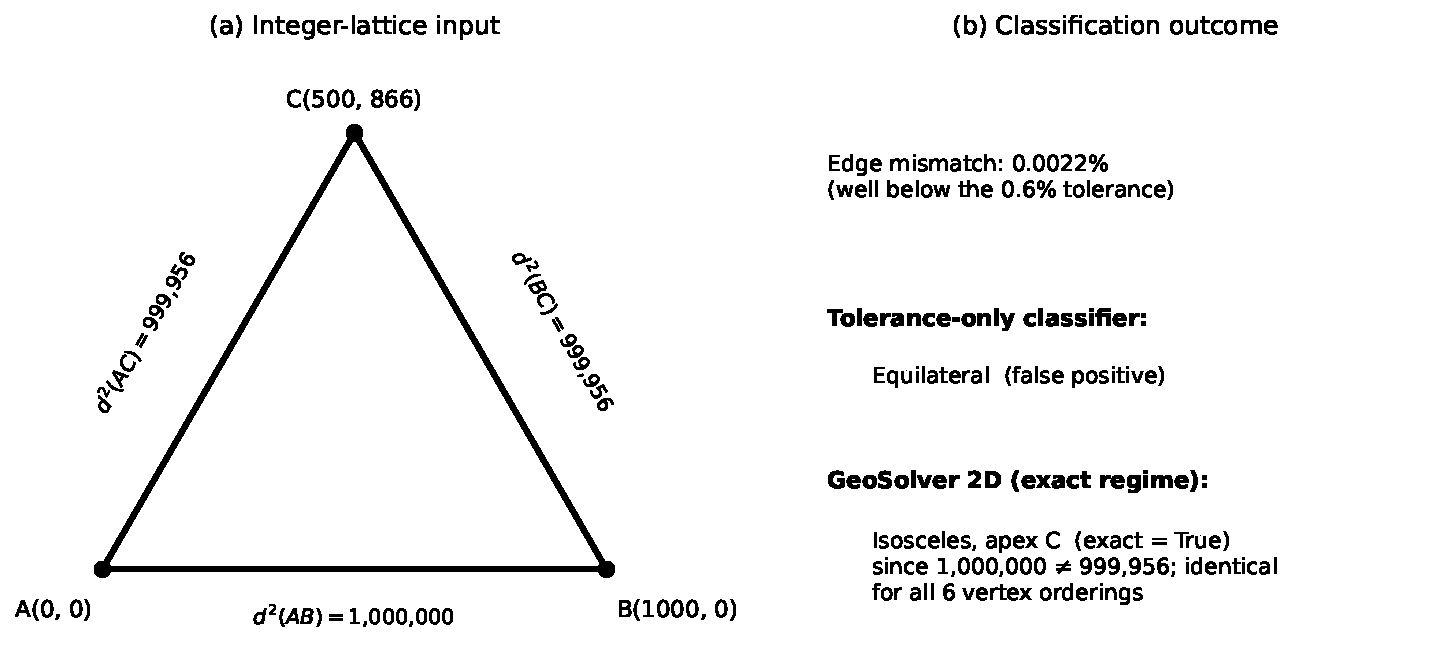
\includegraphics[width=\linewidth]{fig_example1.pdf}
\caption{Schematic of Example 1 (values computed from the stated coordinates; not an application screenshot). (a) The lattice triangle $A(0,0)$, $B(1000,0)$, $C(500,866)$ has squared side lengths $1{,}000{,}000$, $999{,}956$, $999{,}956$. (b) A tolerance-only classifier with $\text{tol\_rel}=0.006$ labels it equilateral; GeoSolver 2D compares the integer squared lengths exactly and reports an isosceles triangle with apex $C$.}
\label{fig:example1}
\end{figure}

\section{Empirical Verification and Sensitivity Analysis}
\label{sec:benchmarks}

\subsection{Tolerance Sensitivity Analysis and Adversarial Stress Tests}
The following experiments verify invariance properties and characterise tolerance sensitivity across continuous and discrete regimes; they are designed to evaluate the operational trade-offs of the relative tolerance parameter ($\mathrm{tol_{rel}}$), not to claim a general recognition accuracy on unconstrained hand drawings. We evaluated a benchmark dataset of 1,000 synthetic triangles (250 each of ground-truth Equilateral, Isosceles, Right, and Scalene prototypes) generated using \texttt{scripts/sensitivity\_benchmark.py} ($\text{seed} = 42$) perturbed by Gaussian coordinate jitter ($\sigma = 0.03$, $0.3\%$ of nominal edge length $10.0$). Table~\ref{tab:canonical} measures the tolerance-versus-noise performance on these continuous prototypes.

\begin{table}[!htbp]
\centering
\caption{Classification performance across continuous prototypes ($\text{tol\_rel} = 0.006$, $\sigma = 0.03$).}
\label{tab:canonical}
\small
\resizebox{\linewidth}{!}{%
\begin{tabular}{@{}lrrrrr@{}}
\toprule
\textbf{Triangle Class} & \textbf{Ground Truth} & \textbf{True Positive (TP)} & \textbf{Recall (\%)} & \textbf{Precision (\%)} & \textbf{F1-Score (\%)} \\
\midrule
Equilateral & 250 & 205 & 82.0\% & 100.0\% & 90.1\% \\
Isosceles & 250 & 212 & 84.8\% & 82.5\% & 83.6\% \\
Right & 250 & 247 & 98.8\% & 100.0\% & 99.4\% \\
Scalene & 250 & 250 & 100.0\% & 85.9\% & 92.4\% \\
\midrule
\textbf{Overall Dataset} & \textbf{1,000} & \textbf{914} & \textbf{91.4\%} & \textbf{91.4\%} & \textbf{91.4\%} \\
\bottomrule
\end{tabular}%
}
\end{table}

\paragraph{Empirical Sensitivity Scan Across Relative Edge Tolerance}
We evaluated empirical sensitivity across relative edge tolerances $\mathrm{tol_{rel}} \in [0.002, 0.010]$:
\begin{itemize}
\item $\text{tol\_rel} = 0.002$: Overall = 62.9\%, Equilateral Recall = 15.2\%, Precision = 100.0\%, Scalene Precision = 55.7\% (overly restrictive; rejects valid hand-drawn regular shapes).
\item $\text{tol\_rel} = 0.004$: Overall = 77.8\%, Equilateral Recall = 47.6\%, Precision = 100.0\%, Scalene Precision = 72.5\%.
\item $\text{tol\_rel} = 0.006$ (Default): Overall = 91.4\%, Equilateral Recall = 82.0\%, Precision = 100.0\%, Scalene Precision = 85.9\% (conservative default for interactive stylus/freehand drawing).
\item $\text{tol\_rel} = 0.008$: Overall = 96.8\%, Equilateral Recall = 92.8\%, Precision = 100.0\%, Scalene Precision = 94.7\%.
\item $\text{tol\_rel} = 0.010$: Overall = 98.5\%, Equilateral Recall = 97.6\%, Precision = 100.0\%, Scalene Precision = 96.5\%.
\end{itemize}

\paragraph{Hard Negatives Stress Test (Near-Boundary Asymmetric Triangles)}
To evaluate robustness against near-boundary false positives across distinct geometric families, we evaluated 200 near-boundary scalene triangles (100 near-isosceles with side mismatch drawn from $0.8\%\text{--}1.5\%$, and 100 near-right with angles in $[88.0^\circ, 88.8^\circ]$ where $|\cos \theta| \in [0.021, 0.035]$), as summarized in Table~\ref{tab:hard_negatives}. These 200 configurations are deliberately designed as adversarial near-boundary test vectors, not representing the natural frequency of shapes in typical student usage.

\begin{table}[!htbp]
\centering
\caption{Hard-negative false-positive rates across relative edge tolerances ($N = 200$).}
\label{tab:hard_negatives}
\small
\resizebox{\linewidth}{!}{%
\begin{tabular}{@{}lrrrrr@{}}
\toprule
$\text{tol\_rel}$ & \textbf{Near-Iso FP} & \textbf{Near-Right FP} & \textbf{Total Scalene TN} & \textbf{Total FP} & \textbf{Combined FP Rate} \\
 & ($N=100$) & ($N=100$) & ($N=200$) & ($N=200$) & (\%) \\
\midrule
0.002 & 0/100 & 0/100 & 200/200 & 0/200 & 0.0\% \\
0.004 & 0/100 & 0/100 & 200/200 & 0/200 & 0.0\% \\
0.006 (Default) & 0/100 & 0/100 & 200/200 & 0/200 & 0.0\% \\
0.008 & 1/100 & 0/100 & 199/200 & 1/200 & 0.5\% \\
0.010 & 36/100 & 0/100 & 164/200 & 36/200 & 18.0\% \\
\bottomrule
\multicolumn{6}{@{}p{\linewidth}@{}}{\footnotesize \textit{Note:} Near-Right FP remains $0/100$ because right-angle classification is governed by the decoupled orthogonal angular tolerance ($|\cos \theta| \le 0.015$), which is held fixed while $\mathrm{tol_{rel}}$ is swept; near-right configurations with $|\cos \theta| \ge 0.021$ correctly remain outside this angular acceptance threshold.}
\end{tabular}%
}
\end{table}

This empirical behavior directly reflects the underlying geometric design: false positives in the near-isosceles family only begin to emerge as $\text{tol\_rel}$ enters and exceeds the $0.8\%\text{--}1.5\%$ perturbation band ($1/100$ at $0.008$, $36/100$ at $0.010$), while the 100 near-right scalene configurations produce $0/100$ false positives across all tolerance levels because the orthogonal classifier employs a decoupled fixed angular bound ($|\cos \theta| \le 0.015$, corresponding to $[89.14^\circ, 90.86^\circ]$).

Fig.~\ref{fig:sensitivity} summarizes the tolerance trade-off: accuracy and equilateral recall increase with $\text{tol\_rel}$, whereas the hard-negative false-positive rate rises sharply above $0.008$.

\begin{figure}[!htbp]
\centering
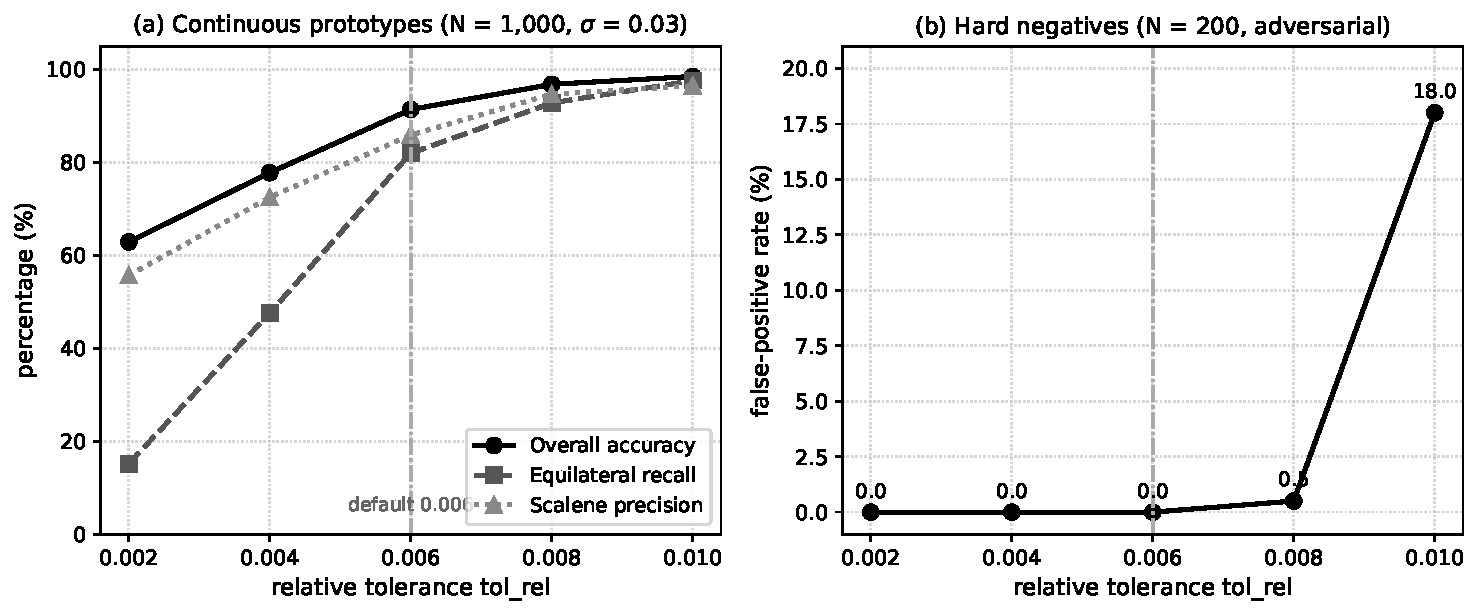
\includegraphics[width=\linewidth]{fig_sensitivity.pdf}
\caption{Tolerance sensitivity, plotted from the values in Tables~\ref{tab:canonical} and~\ref{tab:hard_negatives} and the scan above. (a) Overall accuracy, equilateral recall and scalene precision on the 1,000 continuous prototypes. (b) False-positive rate on the 200 adversarial near-boundary scalene triangles. The dash-dotted line marks the default $\text{tol\_rel}=0.006$.}
\label{fig:sensitivity}
\end{figure}

\paragraph{Empirical Invariance and Comparative Baselines}
\begin{enumerate}
\item \textbf{Permutation Equivariance vs.\ Naive Classifier:} Under a naive positional \texttt{if/elif} classifier evaluated across all $3! = 6$ vertex permutations, apex identification fails to be equivariant whenever competing edges fall within tolerance. On the canonical dataset of 1,000 continuous prototypes in this noise regime ($\sigma = 0.03$, $\mathrm{tol_{rel}} = 0.006$; Table~\ref{tab:canonical}), the naive classifier exhibited apex-variant outcomes on 10.1\% of detected isosceles triangles ($26 / 257$), whereas GeoSolver 2D achieved 0.0\% variance ($0 / 257$). On the 200 adversarial near-tie configurations (constructed specifically where multiple edge pairs satisfy tolerance), the naive classifier produced inconsistent apex assignments in 100.0\% of cases ($200 / 200$), while GeoSolver 2D preserved exact apex equivariance across all instances ($0 / 200$).
\item \textbf{Lattice Exactness on $20 \times 20$ Integer Grid vs.\ Naive Tolerance Classifier:} To quantify the false-positive risk of continuous tolerance classifiers on discrete lattices, we evaluated all $10{,}482{,}124$ non-collinear triangles on the discrete grid $[0, 19]^2$ using \texttt{scripts/lattice\_benchmarks.py}. Under a standard relative tolerance definition ($(\max(s) - \min(s)) / \max(s) \le 0.006$), exactly $116$ configurations satisfy the continuous equilateral criterion. These $116$ triangles fall into two distinct congruence classes: an isosceles class with squared side lengths $(241, 241, 242)$ (e.g., $(0,0), (4,15), (15,4)$, with $0.21\%$ mismatch) and a scalene class with squared lengths $(369, 370, 373)$ (e.g., $(0,0), (3,19), (18,7)$, with $0.54\%$ mismatch). A continuous tolerance classifier falsely labels all $116$ instances as equilateral ($116$ false positives). In contrast, GeoSolver 2D's discrete integer kernel evaluates squared Euclidean distances under exact integer arithmetic, correctly rejecting the equilateral hypothesis across all cases ($0 / 116$ false positives, matching symbolic ground truth in SymPy 1.14~\cite{meurer2017} evaluated across all 116 instances).

On an isolated throughput benchmark on a single x86\_64 CPU core (Python 3.11; reporting median and sample standard deviation $\sigma$ across 10 independent runs of 1,000 evaluations on the 116 near-equilateral lattice triangles), we timed multiple implementations of the equilateral-rejection predicate:
(i) a bare integer squared-length equality check ($d_{12}^2 == d_{23}^2 == d_{31}^2$): $0.68\,\mu\text{s}$ per triangle ($\sigma = 0.09\,\mu\text{s}$);
(ii) exact rational arithmetic via standard \texttt{fractions.Fraction}: $8.62\,\mu\text{s}$ per triangle ($\sigma = 2.07\,\mu\text{s}$);
(iii) GeoSolver 2D headless classification on raw coordinate tuples (\texttt{classify\_triangle}): $7.13\,\mu\text{s}$ per triangle ($\sigma = 1.15\,\mu\text{s}$);
(iv) GeoSolver 2D complete pipeline (including DAG provenance propagation, dynamic taint tracking, and full metadata dictionary generation): $52.12\,\mu\text{s}$ per triangle ($\sigma = 4.82\,\mu\text{s}$); and
(v) symbolic ground truth in SymPy 1.14: $1{,}738\,\mu\text{s}$ per triangle ($\sigma = 142\,\mu\text{s}$).
SymPy is included solely to illustrate the substantial overhead of general-purpose computer algebra systems, not as a practical interactive baseline.
Standard rational arithmetic (\texttt{fractions.Fraction}) is an effective exact alternative for the isolated equality predicate on $\mathbb{Q}^2$. GeoSolver 2D employs $10^k$ decimal-lattice scaling to align directly with fixed-precision GUI input digitizers; its primary scientific contribution is the overall decision architecture---specificity hierarchy, permutation-invariant candidate ranking, apex selection, and provenance propagation---rather than exact arithmetic in isolation. The $52.12\,\mu\text{s}$ latency of full DAG provenance propagation remains negligible within standard $60\,\text{FPS}$ ($16.7\,\text{ms}$) interactive canvas rendering budgets.
\item \textbf{Decimal Lattice Sweep ($k \in \{1, 2, 3, 4\}$):} Across 496 non-collinear candidate pairs evaluated on decimal-scaled lattices where float squared lengths drift at $10^{-16}$, GeoSolver 2D's discrete integer kernel achieved 100.0\% exact recognition ($496/496$: 490 isosceles + 6 right-isosceles, all \texttt{exact=True} with apex at $A$).
\item \textbf{Exhaustive Integer Grid Sweep ($10 \times 10$ Lattice):} To verify the implementation in the discrete regime without sampling bias, we evaluated all non-collinear vertex triples formed by points in the discrete integer grid $[0, 9]^2$ ($157{,}252$ distinct triangles) across all $3! = 6$ vertex orderings ($943{,}512$ total evaluations). As expected from integer arithmetic, zero lattice triangles were classified as equilateral, serving as an implementation sanity check. In this discrete regime on $[0, 9]^2$, no permutation-order or apex-equivariance violations were observed ($0 / 943{,}512$), confirming the label-free sorting implementation.
\end{enumerate}

\subsection{Automated Regression Test Suite}
The codebase was verified using Python's standard \texttt{unittest} framework across 62 tests:
\begin{itemize}
\item \textbf{Headless Core Library Suite (27 tests):} Pure Python standard library, zero GUI dependencies. Automatically executed on GitHub Actions CI across Ubuntu, Windows, and macOS on Python 3.10--3.13. Achieves 92\% statement coverage across \texttt{geosolver\_core} (94\% on \texttt{classifier.py}, 90\% on \texttt{provenance.py}), reproducible via \texttt{python -m coverage run --source=geosolver\_core -m unittest discover tests}. Verifies discrete integer arithmetic, lattice impossibility assertions, scale invariance, adversarial near-tie test vectors, DAG provenance invariants, cycle safety, deep DAG order-independence, stack safety up to 2,000 nodes, 25-level diamond ladder traversal with linear $O(V+E)$ complexity, and integer return types on grid snapping.
\item \textbf{Desktop GUI Canvas Integration Suite (35 tests):} Covers Tkinter canvas event handling, mouse drag snapping, undo/redo instance rebinding, and WCAG 2.1 AA luminance contrast~\cite{wcag21}. All tests are included in the open repository.
\item \textbf{Aggregate Verification Metric:} All 62 unit tests pass successfully ($62 / 62$, 100.0\%).
\item \textbf{Cross-Platform Verification:} Automated CI pipeline (\texttt{.github/workflows/ci.yml}) executes across \texttt{ubuntu-latest}, \texttt{windows-latest}, and \texttt{macos-latest} on Python 3.10 through 3.13.
\end{itemize}

\section{Impact and Practical Applications}

GeoSolver 2D addresses a specific, well-defined gap: interactive geometry tools that classify freehand or lattice-based triangles using tolerance heuristics can return results that depend on vertex order or that contradict exact arithmetic. By making classification permutation-invariant and by evaluating integer-lattice inputs exactly, the kernel is designed to provide consistent, mathematically defensible feedback in two settings:

\begin{itemize}
\item \textbf{Potential Embeddable Micro-Kernel:} Because GeoSolver 2D is implemented in pure Python without external dependencies, it could be embedded as an autograding micro-kernel within online STEM learning environments (e.g., JupyterHub, Moodle, or automated homework graders). No such deployment has yet been evaluated in production; this represents a promising direction for future educational software integration.
\item \textbf{Geometric Modelling Pipelines:} By sorting candidate hypotheses over label-free keys, the classifier ensures that triangle classification is invariant to vertex ordering, which could benefit CAD pre-processors and geometric constraint solvers where input serialization varies.
\end{itemize}

\subsection{Current Use and Limitations}
The educational desktop edition has been distributed through the Microsoft Store. However, we explicitly acknowledge four design and scope limitations:
\begin{enumerate}
\item \textbf{Tolerance Threshold Sensitivity:} The continuous regime inherently depends on a user-adjustable relative tolerance ($\mathrm{tol_{rel}}$). While our candidate ordering eliminates vertex-permutation order dependence, it does not eliminate threshold sensitivity near decision boundaries (Table~\ref{tab:hard_negatives}).
\item \textbf{Scale Transitions across Regimes:} The regime of an untagged input depends on its decimal representation; uniformly scaling $(0,0), (1,0), (0.51, 0.86598)$ by $\times 10$ alters its decimal representation from 5 places to 4 places, moving it from the continuous to the exact regime and changing its classification (Sec.~\ref{sec:dual_regime}). This is a deliberate design choice reflecting the semantic contract that user-entered decimal digits are treated as exact fixed-point specifications, meaning exactness is defined post-quantization on the decimal lattice $\mathbb{Z}^2/10^k$, rather than an inconsistency of Proposition~\ref{prop:invariance}.
\item \textbf{Geometric Scope:} The current kernel is specialized for planar triangles in $\mathbb{R}^2$. Extension to general polygons, conic sections, and 3D spatial geometry remains future work.
\item \textbf{Educational Evaluation:} No classroom evaluation or formal learning-outcome study has been conducted to date; this release focuses entirely on algorithmic correctness, reproducibility, and software reusability.
\end{enumerate}

\section{Conclusions and Future Work}
GeoSolver 2D demonstrates that combining provenance-flag tracking with specificity-ordered predicates addresses the tension between continuous user interaction and discrete mathematical truth. By evaluating exact integer lattice arithmetic when appropriate and sorting candidate hypotheses deterministically under continuous perturbations, the kernel provides intra-regime scale invariance and permutation-invariant classification. The present work validates the classification kernel through automated regression tests and synthetic benchmarks; classroom evaluation and extension to 3D spatial geometry remain future work.

\section*{CRediT Authorship Contribution Statement}
\textbf{Bao-Trung Nguyen}: Conceptualization, Methodology, Software, Validation, Formal analysis, Investigation, Writing -- original draft, Writing -- review \& editing.

\section*{Funding}
This research did not receive any specific grant from funding agencies in the public, commercial, or not-for-profit sectors.

\section*{Declaration of Competing Interest}
The author develops and distributes GeoSolver, an educational dynamic geometry application available on the Microsoft Store, which is currently free of charge. The author has received no revenue from this application to date. As an independent researcher bearing all development and infrastructure costs without institutional support, the author plans to offer an optional paid Pro edition in the future to help sustain ongoing development; this edition has not yet been released. The core mathematical algorithms, classification engine, and provenance tracking system described in this paper are released as free and open-source software under the GNU General Public License v3 (GPLv3), and no part of the described research is gated behind paid features. The author has no other known competing financial interests or personal relationships that could have appeared to influence the work reported in this paper.

\section*{Data Availability}
All source code, automated regression suites (62 tests), and reproducible benchmark scripts are publicly available in the permanent repository at \url{https://github.com/trungyds16-coder/geosolver-core} (release tag \texttt{v3.2.1}) and permanently archived on Zenodo (\href{https://doi.org/10.5281/zenodo.24249595}{DOI: 10.5281/zenodo.24249595}):
\begin{itemize}
\item \texttt{scripts/sensitivity\_benchmark.py}: Reproduces canonical prototype evaluation (Table~\ref{tab:canonical}), empirical sensitivity sweeps across $\mathrm{tol_{rel}}$, hard-negative stress tests (Table~\ref{tab:hard_negatives}), and the natural and adversarial apex-invariance benchmarks (including the $26/257$ and $200/200$ comparisons).
\item \texttt{scripts/lattice\_benchmarks.py}: Reproduces the exhaustive $10 \times 10$ integer grid sweep ($157{,}252$ triangles), the $20 \times 20$ grid evaluation ($116$ continuous false positives), symbolic verification via SymPy 1.14 across all 116 instances, and the multi-baseline throughput benchmark across 10 independent runs.
\item \texttt{examples/autograder.py}: Provides the runnable educational autograder integration (Example 3), validated automatically in continuous integration.
\item \texttt{scripts/make\_figs.py}: Generates publication figures (\texttt{fig\_example1.pdf} and \texttt{fig\_sensitivity.pdf}) directly from benchmark results.
\end{itemize}

\section*{Declaration of Generative AI in Scientific Writing}
During the preparation of this work the author used Claude (Anthropic) and Gemini (Google) in order to assist with code refactoring, test case generation, and manuscript language editing. After using these tools, the author reviewed and edited the content as needed and takes full responsibility for the content of the publication.

% Bibliography
\begin{thebibliography}{11}
\expandafter\ifx\csname natexlab\endcsname\relax\def\natexlab#1{#1}\fi
\providecommand{\url}[1]{\texttt{#1}}
\providecommand{\href}[2]{#2}
\providecommand{\path}[1]{#1}
\providecommand{\doi}[1]{\href{https://doi.org/#1}{#1}}
\providecommand{\DOIprefix}{doi:}
\providecommand{\ArXivprefix}{arXiv:}
\providecommand{\URLprefix}{URL: }
\providecommand{\projecturl}[1]{\url{#1}}

\bibitem[{Jackiw(1995)}]{jackiw1995}
N.~Jackiw, The Geometer's Sketchpad [Computer software], Key Curriculum Press, Berkeley, CA (1995).

\bibitem[{Laborde(2001)}]{laborde2001}
C.~Laborde, Integration of technology in the design of geometry tasks with
  {Cabri-Geometry}, International Journal of Computers for Mathematical Learning
  6~(3) (2001) 283--317. \DOIprefix\doi{10.1023/A:1013309728825}.

\bibitem[{Richter-Gebert and Kortenkamp(1999)}]{cinderella1999}
J.~Richter-Gebert, U.~H. Kortenkamp, The Interactive Geometry Software
  Cinderella, Springer-Verlag, Berlin, Heidelberg (1999).
  \DOIprefix\doi{10.1007/978-3-642-58385-8}.

\bibitem[{Hohenwarter and Jones(2007)}]{hohenwarter2007}
M.~Hohenwarter, K.~Jones, Ways of linking geometry and algebra: The case of
  {GeoGebra}, Proceedings of the British Society for Research into Learning
  Mathematics 27~(3) (2007) 126--131.

\bibitem[{Kettner et~al.(2008)Kettner, Mehlhorn, Pion, Schirra, and Yap}]{kettner2008}
L.~Kettner, K.~Mehlhorn, S.~Pion, S.~Schirra, C.~Yap, Classroom examples of
  robustness problems in geometric computations, Computational Geometry:
  Theory and Applications 40~(1) (2008) 61--78.
  \DOIprefix\doi{10.1016/j.comgeo.2007.06.003}.

\bibitem[{Shewchuk(1997)}]{shewchuk1997}
J.~R. Shewchuk, Adaptive precision floating-point arithmetic and fast robust
  geometric predicates, Discrete \& Computational Geometry 18~(3) (1997)
  305--363. \DOIprefix\doi{10.1007/PL00009321}.

\bibitem[{{The CGAL Project}(2024)}]{cgal2024}
{The CGAL Project}, {CGAL} User and Reference Manual, 5.6 ed., CGAL Editorial
  Board (2024).

\bibitem[{Meurer et~al.(2017)}]{meurer2017}
A.~Meurer, C.~P. Smith, M.~Paprocki, O.~{\v{C}}ert{\'{\i}}k, S.~B. Kirpichev,
  M.~Rocklin, et~al., {SymPy}: symbolic computing in {Python}, PeerJ Computer
  Science 3 (2017) e103. \DOIprefix\doi{10.7717/peerj-cs.103}.

\bibitem[{Schwartz et~al.(2010)Schwartz, Avgerinos, and Brumley}]{schwartz2010}
E.~J. Schwartz, T.~Avgerinos, D.~Brumley, All you ever wanted to know about
  dynamic taint analysis and forward symbolic execution (but might have been
  afraid to ask), in: Proceedings of the IEEE Symposium on Security and Privacy
  (S\&P 2010), 2010, pp. 317--331. \DOIprefix\doi{10.1109/SP.2010.26}.

\bibitem[{{IEEE Computer Society}(2019)}]{ieee754}
{IEEE Computer Society}, {IEEE} Standard for Floating-Point Arithmetic,
  Standard IEEE Std 754-2019, IEEE (2019) 1--84.
  \DOIprefix\doi{10.1109/IEEESTD.2019.8766229}.

\bibitem[{{World Wide Web Consortium (W3C)}(2018)}]{wcag21}
{World Wide Web Consortium (W3C)}, Web content accessibility guidelines
  ({WCAG}) 2.1, W3C Recommendation, W3C (2018).

\end{thebibliography}

\end{document}
